\chapter{Grundlagen} \label{ch:background}

\begin{center}
    \textit{Was Objekt Detektion ausmacht - finden und klassifizieren}
\end{center}

Im Bereich Computer Vision ist die Objekt Detektion eines der schwierigsten fundamentalen Probleme \cite{szeliski_computer_2010}.
Folgende Unterprobleme werden in \autoref{ch2:fig:cv_problems} veranschaulicht:
\begin{itemize}
    \item \textbf{Klassifikation}: semantische Gruppe einem Bild zuweisen
    \item \textbf{Lokalisation}: Postion einer semantischen Gruppe im Bild finden
    \item \textbf{Detektion}: mehrere semantische Gruppen im Bild finden
    \item \textbf{Segmentation}: pixelgenaue Gruppenbestimmung eines Bildes
\end{itemize}

\begin{figure}[ht]
    \centering
    \subfloat[{\color{black}Katze}]{{\includegraphics[height=.35\textwidth]{figures/cv_problems/classification}}}
    \subfloat[{\color{black}Katze}]{{\includegraphics[height=.35\textwidth]{figures/cv_problems/lokalization}}}
    \subfloat[{\color{Maroon}Person}, {\color{RoyalBlue}Hund}]{{\includegraphics[height=.35\textwidth]{figures/cv_problems/detection}}}
    \subfloat[{\color{Maroon}Person}, {\color{RoyalBlue}Hund}]{{\includegraphics[height=.35\textwidth]{figures/cv_problems/segmentation}}}
    \caption[Unterprobleme der visuellen Bildverarbeitung]{Unterprobleme in der visuellen Bildverarbeitung. Von links nach rechts: Klassifikation, Lokalisation, Detektion, Segmentation}
    \label{ch2:fig:cv_problems}
\end{figure}

Inhalt dieser Arbeit ist die Objekt Detektion, da alle Traktoren in einem Bild gefunden und klassifiziert werden sollen.
Eine typische Objekt Detektion Pipeline setzt sich zusammen aus \cite{wu_recent_2019}:
\begin{enumerate}
    \item \textbf{\acp{ROI} bestimmen}:
        Bereiche im Bild finden, welche Objekte enthalten.
        Die intuitive Herangehensweise, mit einem \gls{sliding} das gesamte Bild abzutasten, resultiert dabei in langen Laufzeiten.
    \item \textbf{Feature Vector Extraction}:
        Anschließend werden mittels verschiedener Filter die Bildinformation der jeweiligen \ac{ROI} extrahiert.
    \item \textbf{Region Klassifikation}:
        Im letzten Schritt werden dem Feature Vector kategorische Label zugewiesen und so die Klasse der Region bestimmt.
\end{enumerate} 

Nachstehend werden diese drei Schritte genauer beleuchtet:
\autoref{ch2:bgs} beschäftigt sich damit, wie die \acp{ROI} mittels \nameref{ch2:bgs} bestimmt werden können, und \autoref{ch2:cnn} beschreibt, wie die gefundenen \acp{ROI} einer Klasse zugewiesen werden.
Zur Feature Extraktion und Klassifikation werden \acp{CNN} verwendet.
Diese beruhen auf \acp{ANN}, welche in \autoref{ch2:ann} eingeführt werden.

% -------------------------------------------------

\section{Background Subtraction} \label{ch2:bgs}

\begin{center}
    \textit{Wie Bewegungen in Bildsequenzen erkannt werden}
\end{center}

Bei der Verwendung von statischen Kameras ist Background Subtraction einer der meistbenutzten Ansätze zur Erkennung von Änderungen in Bildsequenzen \cite{goyette_changedetection.net:_2012}.
Dabei soll das Eingangsbild in Vordergrund und Hintergrund unterteilt werden.

In der einfachsten Vorgehensweise wird zuerst ein Hintergrundbild aufgenommen, das keine bewegenden Objekte enthält. 
Im nächsten Schritt wird die Differenz von Hintergrundbild $BG$ und Bild $F_n$ berechnet.
Jedes Pixel $x$, das eine höhere Differenz als Schwellwert $\tau$ aufweist, wird als Vordergrund markiert.
\begin{flalign}
    K(x) = 
    \begin{cases}
        1, & \text{falls}\ |BG(x) - F_n(x)| > \tau \\
        0, & \text{sonst.}
    \end{cases}
\end{flalign}

Das setzt jedoch ein Hintergrundbild voraus und ist anfällig für Lichtveränderungen, neue Objekte oder entfernte Objekte \cite{maddalena_background_2012}.

Die meisten Ansätze erstellen deshalb ein Background Modell aus den ersten $N$ Bildern \textit{(Background Initialization)} und passen dieses stetig an \textit{(Background Maintenance)} \cite{maddalena_background_2012, yao_comparative_2017,sobral_comprehensive_2014}. 
Anschließend wird aus Bild $F_n$ und Background Modell eine Vordergrundmaske $M_n$ erstellt \textit{(Foreground Detection)}.
Die Konturen in $M_n$ bilden die \acp{ROI} ab.

Die Methoden, um ein Background Modell zu erstellen und zu pflegen, lassen sich grob in \textit{Basic Models, Statistical Models, Background Estimation, Background Clustering und Neural Network Modeling} gliedern \cite{goyal_review_2018}. 
Die spezifische Methode, für die sich in dieser Arbeit entschieden wurde, ist in \autoref{ch3:bmog} beschrieben.

\bigskip
Im, in \autoref{ch2:fig:bgs} dargestellten, Beispiel ergeben sich aus der Vordergrundmaske zwei \acp{ROI}.
Handelt es sich allerdings beim Eingangsbild um eine komplexere Szenerie mit beispielsweise Schattenwurf einer Wolke, werden zusätzliche Bewegungen detektiert.
Diese sind für unseren Anwendungsfall nicht interessant und müssen gesondert behandelt werden.
Deshalb gilt es die gefundenen Regionen zu klassifizieren.

\begin{figure}[ht]
    \centering
    \subfloat[Eingangsbild $F$]{{\includegraphics[width=.33\textwidth]{figures/bg_subtraction/2_in}}}
    \subfloat[Vordergrundmaske $M$]{{\includegraphics[width=.33\textwidth]{figures/bg_subtraction/2_fg}}}
    \subfloat[Background Model]{{\includegraphics[width=.33\textwidth]{figures/bg_subtraction/2_bg}}}
    \caption{Background Subtraction Beispiel}
    \label{ch2:fig:bgs}
\end{figure}

% -------------------------------------------------

\section{Artificial Neural Networks} \label{ch2:ann}

\begin{center}
    \textit{Wie Computer - inspiriert vom biologischen Gehirn - lernen können}
\end{center}

\acp{ANN} sind eine Machine Learning Technik, welche auf unserem Verständnis biologischer Neuronaler Netze beruht.
Dabei soll - wie beim menschlichen Gehirn - aus vorherigen Erfahrungen gelernt werden.
\citeauthor{mitchell_machine_1997} definiert Maschinelles Lernen wie folgt \cite{mitchell_machine_1997}: 

\begin{quotation}
\textit{A computer program is said to learn from experience E with respect to some class of tasks T and performance measure P, if its performance at tasks in T, as measured by P, improves the experience E.}
\end{quotation}

\textit{Task $T$} beschreibt in unserem Anwendungsfall das Klassifizieren von Landmaschinen, während \textit{performance measure $P$} zum Beispiel die Genauigkeit der Klassifikation meint.
\textit{Experience $E$} sind die Eingangsbilder (\ac{ROI}), welche zum Lernen genutzt werden.
Das erwartete Ergebnis von $E$ ist bekannt, weshalb man von \gls{supervised} spricht.

% -------------------------------------------------
\subsection{Perzeptron}
Die Grundeinheit eines jeden \ac{ANN}s bildet das Perzeptron (zu sehen in \autoref{ch2:fig:perceptron}). 

\begin{figure}[ht]
    \center
    \input{tiks/perceptron-unit.tex}
    \caption{Einfaches Perzeptron (nach \cite{noauthor_martinthoma/latex-examples_nodate})}
    \label{ch2:fig:perceptron}
\end{figure}

Es hat mehrere Eingaben ($x_1, x_2, .., x_n$) und eine Ausgabe $y$.
Zusätzlich hat es einen Bias $x_0$. Jede Eingabe wird mit den Gewichtungen ($w_0, w_1, .., w_n$) multipliziert.
Anschließend entscheidet die Aktivierungsfunktion $\sigma$ darüber, wie stark das Perzeptron feuert:
\begin{flalign}
    y &= \sigma
        \left( 
            { \sum_{i=0}^{n} x_i \cdot w_i } 
        \right)
\end{flalign}

Der Bias ermöglicht eine Verschiebung der Aktivierung.
Eine der vielen Aktivierungsfunktionen $\sigma$ ist die einfache Heaviside Funktion, welche für jede beliebige negative Zahl den Wert Null und andernfalls Eins hat:
\begin{flalign}
    \sigma(z) &=
        \begin{cases}
            1, & \text{falls}\ z \geq 0 \\
            0, & \text{sonst.}
        \end{cases}
\end{flalign}

Die drei am häufig genutzten Aktivierungsfunktionen sind in \autoref{ch2:fig:activation} zu sehen.

\begin{figure}[ht]
    \begin{small}
        \begin{center}
            \pgfplotsset{every axis/.append style={tick label style={/pgf/number format/fixed},font=\scriptsize,ylabel near ticks,xlabel near ticks,grid=major}}

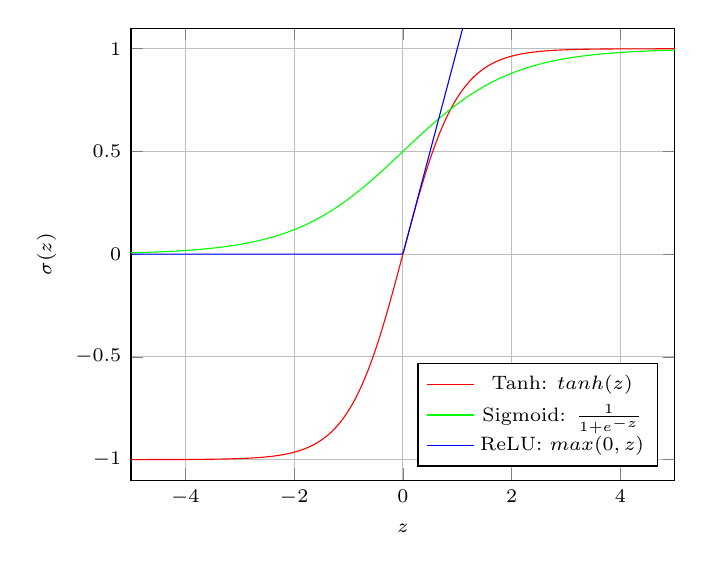
\begin{tikzpicture}
    \begin{axis}[width=0.7\textwidth,ylabel=$\sigma(z)$,xlabel=$z$,ymin=-1.1,ymax=1.1,xmin=-5,xmax=5,legend pos=south east, samples=300]
        \addplot[red,smooth] {tanh(x)};
        \addplot[green,smooth] {1/(1+exp(-x))};
        \addplot[blue,smooth] {max(0,x)};
        \addlegendentry{Tanh: $tanh(z)$}
        \addlegendentry{Sigmoid: $\frac{1}{1+e^{-z}}$}
        \addlegendentry{ReLU: $max(0, z)$}
    \end{axis}
\end{tikzpicture}
        \end{center}
        \caption{Aktivierungsfunktionen}
        \label{ch2:fig:activation}
    \end{small}
\end{figure}


\subsection{Netzwerk}
In einem \ac{ANN} werden mehrere Perzeptronen zu einem Netzwerk zusammengefügt.
\autoref{ch2:fig:multilayer} zeigt ein solches Netzwerk, welches auch \ac{MLP} genannt wird.
Für jede Verbindung (Pfeil) gib es ein Gewicht.
Das \ac{ANN} besteht aus unterschiedlichen Layern, welche spezifische Namen haben.
Der erste wird \textit{Input} Layer genannt und nimmt die Eingabewerte entgegen; der \textit{Output} Layer liefert die Vorhersage.
Die Layer dazwischen bezeichnet man als \textit{Hidden Layer}. 
Besteht das \ac{ANN} aus mehreren Hidden Layern, handelt es sich um ein tiefes neuronales Netz (engl. Deep Neural Network).

\begin{figure}[ht]
    \center
    \input{tiks/multilayer-perceptron.tex}
    \caption{Multilayer Perzeptron \cite{noauthor_davidstutz/latex-resources_nodate}}
    \label{ch2:fig:multilayer}
\end{figure}

Ein einzelner Layer kann als folgende Funktion $f^l(X)=W^l * f^{l-1}(X) = Y_l$ repräsentiert werden.
Die Gewichte $W^l$ sind die Verbindungen zwischen Layer $l$ und vorangegangenem Layer $l-1$; $Y_l$ bezeichnet die Ausgaben des jeweiligen Layers.

Die Berechnung des gesamten \ac{MLP} wird \textit{Feedforward} genannt.
Das Ergebnis des vorherigen Layers wird hierbei als Eingabewert an den nächsten Layer übergeben (siehe \autoref{ch2:math:feedforward}).
\begin{flalign}
    \label{ch2:math:feedforward}
    f(x) &= f^{L+1}(...(f^2(f^1(x)))
\end{flalign}

Die Ausgabe des letzten Layers wird oft durch eine Softmax-Funktion bestimmt.
Diese führt eine Normalisierung durch, sodass eine Wahrscheinlichkeitsverteilung der Klassen entsteht.

Ist jedes Perzeptron eines Layer mit allen Perzeptron des vorherigen Layers verbunden, spricht man von einem \ac{FC} Layer.
Die Anzahl der zu lernenden Gewichte $W$ kann dabei - je nach Tiefe und Breite des Netzwerks - schnell im Millionenbereich liegen.


Die Motivation für komplexe Netzwerke ist, dass im erstem Layer einfache Muster gefunden werden können.
Basierend auf den einfachen Mustern kann der zweite Layer komplexere Muster finden.
Diese Komplexität nimmt mit jedem Layer zu, sodass in den späteren Layern komplexere Zusammenhänge erkannt werden können.

Eine feste Regel, wie viele Layer benötigt werden, gibt es nicht.
Dies muss durch Ausprobieren bestimmt werden.\footnote{Eine Intuition für verschiedene Konfigurationen kann unter \url{https://playground.tensorflow.org} geschaffen werden (besucht am 10.01.2020).}
Sobald mehrere Hidden Layer verwendet werden, spricht man von Deep \ac{ANN}.

\subsection{Training}
\textit{Backpropagation} \cite{rumelhart_learning_1986} ist die bevorzugte Methode, um \acp{ANN} lernen zu lassen.
Dabei wird ein Trainingsbeispiel, bestehend aus Eingabe $X$ und Zielwert $y$, vom \ac{MLP} berechnet.
Die Vorhersage $\bar y$ wird mit dem Zielwert $y$ verglichen.
Die Abweichung der zwei Werte ist der \textit{Loss} $L$.
Sind die Vorhersagen gut, ist der Loss niedrig und sind die Vorhersagen schlecht, ist der Loss hoch.

Für binäre Klassifikationsprobleme kann die \textit{Binary Cross-Entropy Lossfunktion} verwendet werden.
\begin{flalign}
    loss(y, \bar y) &= - (y \cdot log(\bar y) + (1-y) \cdot log(1- \bar y))
\end{flalign}
Beispielhaft sei $y=1$ und Vorhersage $\bar y=0.9$, so ergibt sich ein niedriger Loss von $0.046$.
Wäre der tatsächliche Wert hingegen $y=0$ gewesen, ist der Loss dementsprechend höher.
\begin{flalign}
    loss(1, 0.9)    &= - (1 \cdot log(0.9) + (1-1) \cdot log(1-0.9)) \\
                    &= - (1 \cdot log(0.9) + \cancel{0 \cdot log(1-0.9)})  \nonumber\\
                    &= 0.046 \nonumber \\
    loss(0, 0.9)    &= - (0 \cdot log(0.9) + (1-0) \cdot log(1-0.9)) \\
                    &= - (\cancel{0 \cdot log(0.9)} + 1 \cdot log(1-0.9)) \nonumber \\
                    &= 1 \nonumber
\end{flalign}

Innerhalb des Lernprozesses soll $L$ minimiert werden.
Dies geschieht, indem die Gewichte des Netzes angepasst werden.
Zur Anpassung wird die partielle Ableitung $\frac{\delta L_i}{\delta w_{kj}}$ von der Lossfunktion und des jeweiligen Gewichtes $w$ gebildet.
Die Ableitung drückt aus, wie stark das Gewicht den Loss beeinflusst.
Um den Loss zu verringern, muss das Gewicht entgegen des Gradienten \textit{gerückt} werden \textit{(Gradient Descent)}.
In welchem Ausmaß die Gewichte angepasst werden, hängt von der \textit{Learningrate} $\alpha$ ab.

Backpropagation erlaubt eine effiziente Bestimmung aller Gradienten.
Dank der Struktur von \acp{ANN} kann zum Ableiten die Kettenregel angewandt werden.
Dazu werden vom Output Layer ausgehend die Gradienten bestimmt und rückwärts durch das Netzwerk \textit{propagiert} (woher der Algorithmus auch seinen Namen hat) \cite{lecun_deep_2015}.
Aufbauend darauf werden die Gradienten der darunterliegenden Layer bestimmt.
Ein Beweis und die vollständige Funktionsweise ist in \citetitle{nielsen_neural_2018} zu finden \cite{nielsen_neural_2018}.

Beim \IT{Stochastic Gradient Descent} wird der Loss nicht für ein Beispiel sondern mehrere berechnet und anschließend die Gradienten nur einmal für diesen \IT{Batch} bestimmt.
Dadurch wird das Training beschleunigt.

\bigskip
Ein einzelner Durchlauf aller Trainingsdaten wird Epoche genannt, wobei ein \ac{ANN} typischerweise mehrere Epochen trainiert.
\autoref{ch2:fig:gradient} zeigt eine Visualisierung des Trainingsprozesses.
Dabei wird die Fehleroberfläche abgebildet. Die roten Punkte markieren die Prediction-Fehler nach jeder Epoche und nähern sich im Laufe des Trainings einem lokalem Minimum an.
\begin{figure}[ht]
    \begin{small}
        \begin{center}
            \includegraphics[width=0.95\textwidth]{figures/gradient_descent_problems-dotted}
        \end{center}
        \caption{Visualisierung des Trainingsprozesses \cite{singh_optimization_2019}}
        \label{ch2:fig:gradient}
    \end{small}
\end{figure}


\subsection{Probleme}
Beim Trainieren eines \ac{ANN}s können folgende Probleme auftreten:
\begin{description}
    \item[Lokale Optima] 
    \autoref{ch2:fig:gradient} zeigt die Fehleroberfläche eines \ac{ANN}.
    Sie hat mehrere lokale Minima sowie Maxima.
    Bei einem Minimum hat jeder umliegende Punkt höhere Kosten, sodass jede kleine Anpassung des Gradienten in einem Anstieg des Fehlerwertes/der Fehlerfunktion resultiert. Dies wirkt sich negativ auf den Trainingsfortschritt aus, da der Algorithmus im lokalen Minimum stecken bleibt.
    So kann es passieren, dass das globale Minimum nicht gefunden wird.
    Sattelpunkte stellen ein ähnliches Problem dar, sollen allerdings unter Verwendung eines Momentum übersprungen werden.

    In der Praxis sind lokale Minima selten ein Problem, da große Netze fast immer ein ähnlich gutes Ergebnis erreichen \cite{lecun_deep_2015}.

    \item[Vanishing Gradients] 
    Durch die Kettenregel werden Gradienten mit den nächsten Layern multipliziert.
    Gradienten, die $<1$ sind, verringern den Gradienten des nächsten Layers.
    Bei tiefen Netzen kann es so vorkommen, dass die Gradienten gegen $0$ gehen je weiter vom Output Layer zum Input Layer durchpropagiert wird. 
    Dadurch machen Vanishing Gradients es unmöglich, die Gewichte bis zum Input Layer anzupassen \cite{goodfellow_deep_2016}.
\end{description}

Allgemeine Probleme im Bereich Machine Learning sind außerdem:
\begin{description}
    \item[Overfitting]
    Das entstandene Modell ist zu sehr auf die gelernten Daten angepasst und generalisiert nicht.
    Es hat die vorhandenen Daten mitsamt Störungen auswendig und kein allgemeines Modell gelernt.
    Dadurch erzielt es auf neuen Daten schlechte Ergebnisse.

    \item[Underfitting]
    Das Modell zeigt das gegenteilige Verhalten zum Overfitting: Es generalisiert zu stark und folgt einem allgemeinem Trend.
    Dieses Phänomen kann mehrere Ursachen haben.
    Darunter fallen zu wenige Trainingsdaten, zu wenige Epochen, zu niedrige Lernrate oder auch ein zu einfaches Modell, wenn dieses zum Beispiel zu wenige Hidden Layer besitzt.
\end{description}

\subsection*{Zusammenfassung}
\ac{ANN} beschreiben eine Technik, bei der der Computer aus Daten lernt.
Sie basieren lose auf dem Konzept des biologischen Gehirns.
Dabei werden Perzeptronen miteinander verbunden.
Das Hintereinanderschalten von Perzeptronen ermöglicht es komplexe Probleme zu lösen.
Je mehr Layer verwendet werden, desto komplexere Probleme kann es lösen.

Gelernt wird, indem das Netzwerk kontinuierlich eine Aufgabe löst und dabei seine Verbindungen (Gewichte) anpasst.

\bigskip
Eine tiefgreifendere theoretische Erklärung ist in \citetitle{goodfellow_deep_2016} von \citeauthor{goodfellow_deep_2016} zu finden.
\citeauthor{nielsen_neural_2018} erklärt in seinem Buch \citetitle{nielsen_neural_2018}, wie die zugrundeliegenden Funktionen programmiertechnisch umgesetzt werden können.
\citeauthor{ng_maschinelles_nodate} lehrt in seinem Onlinekurs eine grundlegende und praxisorientierte Einführung in Machine Learning \cite{ng_maschinelles_nodate}.

% -------------------------------------------------

\section{Convolutional Neural Networks} \label{ch2:cnn}

\begin{center}
    \textit{Wie Muster im Bild automatisch erkannt und gedeutet werden}
\end{center}

\acp{CNN} basieren auf dem Zusammenspiel von \acp{ANN} und Convolutions. 
Ähnlich wie ein \ac{ANN} besteht es aus Neuronen, Gewichten und Bias.
Jedes Neuron erhält eine Eingabe, multipliziert diese mit seinen Gewichten und gibt eine Ausgabe.
Jedoch werden anstatt der \ac{FC} Layer nun Convolutional Layer eingesetzt (Genaueres in \autoref{ch2:cnn:conv}).
So werden die Farbwerte der Pixel auf der einen Seite durch Convolutional Layer verarbeitet und zusammengefasst, sodass ein Klassenwert am anderem Ende vorhersagt wird.
Eingeführt wurden \acp{CNN} bereits \citeyear{lecun_gradient-based_1998}, sind aber erst seit \citeyear{krizhevsky_imagenet_2012} effektiv im Einsatz \cite{lecun_gradient-based_1998,krizhevsky_imagenet_2012,russakovsky_imagenet_2015}.
Ihre neue Popularität verdanken sie den wachsenden Datensammlungen, sowie den weiter steigenden Rechenkapazitäten.

\bigskip
In einem \ac{CNN} ersetzen Convolutions mindestens einen Layer des klassischen \ac{ANN}s und bilden somit den \textit{Convolutional Layer} \cite{goodfellow_deep_2016}.
Zudem werden \textit{Pooling Layer} eingesetzt, um die Dimension der Eingabe zu reduzieren.
Typischerweise sind die Output Layer \ac{FC} und berechnen einen Klassenwert.

\autoref{ch2:fig:cnn} zeigt ein beispielhaftes \ac{CNN}.
Es besteht aus jeweils zwei Convolutional, Pooling und \ac{FC} Layern.
Die einzelnen Layer werden in \autoref{ch2:cnn:conv} und \autoref{ch2:cnn:pool} beschrieben.

\begin{figure}[ht]
    \begin{small}
        \begin{center}
            \includegraphics[width=0.95\textwidth]{figures/simple_cnn}
        \end{center}
        \caption{Einfaches CNN (nach \cite{brilliant_convolutional_nodate})}
        \label{ch2:fig:cnn}
    \end{small}
\end{figure}


\subsection{Convolutions}
\label{ch2:cnn:conv}
Convolutions (auch Filter, Kernel oder Faltung genannt) sind ein verbreitetes Werkzeug in der Bildverarbeitung und werden beispielsweise zum Erkennen von Kanten \textit{(Prewitt, Laplace, Sobel)} oder zum Weichzeichnen \textit{(Box, Gaussian)} eingesetzt.

Eine 2D Convolution ist in \autoref{ch2:fig:2dconv} zu sehen.
Auf das Eingangsbild $I$ wird der Kernel $K$ angewandt und es entsteht eine \textit{Feature Map $F$}.

\begin{figure}[ht]
    \begin{small}
        \begin{center}
            \usetikzlibrary{matrix, positioning}

\definecolor{c1}{HTML}{9ACFC6}
\definecolor{c2}{HTML}{DABBD6}
\definecolor{c3}{HTML}{CBDCB9}
\definecolor{c4}{HTML}{9AC3E1}
\definecolor{c5}{HTML}{DEBBA5}
\definecolor{c6}{HTML}{C4DDE5}

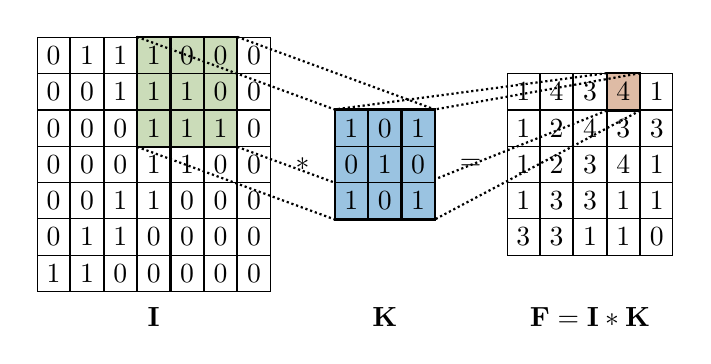
\begin{tikzpicture}
	\matrix (mtr) [matrix of nodes,row sep=-\pgflinewidth, nodes={draw}]
	{
		0 & 1 & 1 & |[fill=c3]| 1 & |[fill=c3]| 0 & |[fill=c3]| 0 & 0\\
		0 & 0 & 1 & |[fill=c3]| 1 & |[fill=c3]| 1 & |[fill=c3]| 0 & 0\\
		0 & 0 & 0 & |[fill=c3]| 1 & |[fill=c3]| 1 & |[fill=c3]| 1 & 0\\
		0 & 0 & 0 & 1 & 1 & 0 & 0\\
		0 & 0 & 1 & 1 & 0 & 0 & 0\\
		0 & 1 & 1 & 0 & 0 & 0 & 0\\
		1 & 1 & 0 & 0 & 0 & 0 & 0\\
	};

	\draw[thick, black] (mtr-1-4.north west) rectangle (mtr-3-6.south east);

	\node [below= of mtr-5-4.south] (lm) {$\bf I$};

	\node[right = 0.2em of mtr] (str) {$*$};

	\matrix (K) [right=0.2em of str,matrix of nodes,row sep=-\pgflinewidth, nodes={draw, fill=c1}]
	{
		1 & 0 & 1 \\
		0 & 1 & 0 \\
		1 & 0 & 1 \\
	};
	\node [below = of K-3-2.south] (lk) {$\bf K$};

	\node [right = 0.2em of K] (eq) {$=$};

	\matrix (ret) [right=0.2em of eq,matrix of nodes,row sep=-\pgflinewidth, nodes={draw}]
	{
		1 & 4 & 3 & |[fill=c5]| 4 & 1\\
		1 & 2 & 4 & 3 & 3\\
		1 & 2 & 3 & 4 & 1\\
		1 & 3 & 3 & 1 & 1\\
		3 & 3 & 1 & 1 & 0\\
	};
	\node [below = of ret-4-3.south] (lim) {${\bf F} = {\bf I} * {\bf K}$};

	\draw[thick, black] (ret-1-4.north west) rectangle (ret-1-4.south east);

	\draw[densely dotted, black, thick] (mtr-1-4.north west) -- (K-1-1.north west);
	\draw[densely dotted, black, thick] (mtr-3-4.south west) -- (K-3-1.south west);
	\draw[densely dotted, black, thick] (mtr-1-6.north east) -- (K-1-3.north east);
	\draw[densely dotted, black, thick] (mtr-3-6.south east) -- (K-3-3.south east);

	\draw[densely dotted, black, thick] (ret-1-4.north west) -- (K-1-1.north west);
	\draw[densely dotted, black, thick] (ret-1-4.south west) -- (K-3-1.south west);
	\draw[densely dotted, black, thick] (ret-1-4.north east) -- (K-1-3.north east);
	\draw[densely dotted, black, thick] (ret-1-4.south east) -- (K-3-3.south east);

	\matrix (K) [right=0.2em of str,matrix of nodes,row sep=-\pgflinewidth, nodes={draw, fill=c4}]
	{
		1 & 0 & 1 \\
		0 & 1 & 0 \\
		1 & 0 & 1 \\
	};

	\draw[thick, black] (K-1-1.north west) rectangle (K-3-3.south east);

	% \node[anchor=south east, inner sep=0.01em, blue] at (mtr-1-4.south east) (xx) {\scalebox{.5}{$\times 1$}};
	% \node[anchor=south east, inner sep=0.01em, blue] at (mtr-1-5.south east) (xx) {\scalebox{.5}{$\times 0$}};
	% \node[anchor=south east, inner sep=0.01em, blue] at (mtr-1-6.south east) (xx) {\scalebox{.5}{$\times 1$}};
	% \node[anchor=south east, inner sep=0.01em, blue] at (mtr-2-4.south east) (xx) {\scalebox{.5}{$\times 0$}};
	% \node[anchor=south east, inner sep=0.01em, blue] at (mtr-2-5.south east) (xx) {\scalebox{.5}{$\times 1$}};
	% \node[anchor=south east, inner sep=0.01em, blue] at (mtr-2-6.south east) (xx) {\scalebox{.5}{$\times 0$}};
	% \node[anchor=south east, inner sep=0.01em, blue] at (mtr-3-4.south east) (xx) {\scalebox{.5}{$\times 1$}};
	% \node[anchor=south east, inner sep=0.01em, blue] at (mtr-3-5.south east) (xx) {\scalebox{.5}{$\times 0$}};
	% \node[anchor=south east, inner sep=0.01em, blue] at (mtr-3-6.south east) (xx) {\scalebox{.5}{$\times 1$}};

\end{tikzpicture}
        \end{center}
        \caption{2D Convolution \cite{velickovic_petarv-/tikz_2019}}
        \label{ch2:fig:2dconv}
    \end{small}
\end{figure}

Im Gegensatz zum \ac{FC} Layer sind bei einem Convolutional Layer nicht alle Eingaben mit jedem Neuron verbunden, sondern nur kleine regionale Ausschnitte \textit{(Local Receptive Fields)}.
Das kleine Sichtfeld wird über die gesamte Eingabe geschoben - vergleichbar mit dem \gls{sliding}.
Aus dem Sichtfeld und dem Kernel wird das Skalarprodukt gebildet.

Für eine Feature Map wird nur ein Kernel verwendet. Das hat zwei Gründe:
\begin{enumerate}[i)]
    \item Das Feature (z.B. eine vertikale Kante) wird überall im Bild erkannt, auch bei Translationen (Verschiebungen).
    Da mehrere Features (z.B. auch horizontale Kanten) erkannt werden sollen, werden in der Praxis mehrere Feature Maps pro Layer erstellt.
    \item Die gleichen Gewichte werden für mehrere Neuronen geteilt. Das schränkt den Parameterraum stark ein \textit{(Weight Sharing)}.
\end{enumerate}

Mathematisch wird für das $j,k$te Neuron die Summe aus den Gewichten des Kernels und des Sichtfelds von $j,k$ gebildet \cite{nielsen_neural_2018}:
\begin{flalign}
    z = (I*K)_{j,k} &= 
        \omega_0 + \sum_{l=0}^{K_{size}} \sum_{m=0}^{K_{size}} \omega_{l,m} \cdot i_{j+l,k+m} \\
    y_{j,k} &= \sigma (z)
\end{flalign}
$\sigma$ denotiert wie zuvor die Aktivierungsfunktion; $\omega_0$ den Bias.
$\omega_{l,m}$ sind die geteilten Gewichte des Kernels, welcher eine Größe von $K_{size} \times K_{size}$ hat.
Die Eingabe $i_{x,y}$ ist das jeweilige Sichtfeld von $I$.

\bigskip
Wie beim \ac{ANN} werden die Gewichte $\omega$ selbstständig erlernt.
In der Trainingsphase wird dementsprechend gelernt, ein Muster zu erkennen; während in der Testphase geschaut wird, ob dieses Muster existiert.
Das ersetzt die historisch sehr aufwändige und eingeschränkte händische Feature Extraktion.

Weitere wichtige Eigenschaften sind:
\begin{itemize}
    \item \textbf{Padding}:
    Wie in \autoref{ch2:fig:2dconv} zu sehen, verkleinert sich die Feature Map von $7 \times 7$ auf $5 \times 5$.
    Das liegt daran, dass der Kernel nur auf $25$ Positionen vollständig passt.
    Um diesen Effekt zu verhindern, kann der Input mit Hilfe von \textit{Padding} erweitert werden. 
    So wird zum Beispiel beim Zero-Padding ein Rand aus Nullen um das Eingangsbild hinzugefügt.
    \item \textbf{Stride}:
    In \autoref{ch2:fig:2dconv} wird das Sichtfeld um jeweils einen Pixel verschoben. Wird das Sichtfeld um $2$ Pixel verschoben, spricht man von einem Stride der Länge $2$. Dadurch würde sich die Feature Map weiter verkleinern.
\end{itemize}

\subsection{Pooling} \label{ch2:cnn:pool}
Nach mehreren Convolutional Layern wird häufig ein Pooling Layer angewandt.
Seine Aufgabe ist es, die Größe der Feature Map zu reduzieren.

\autoref{ch2:fig:pooling} zeigt eine Max-Pooling Operation mit einer Stride- und Filtergröße von $2 \times 2$. Dabei wird der Maximalwert der Region übernommen.
Der Ablauf für ein Average-Pooling ist analog.

\begin{figure}[ht]
    \begin{small}
        \begin{center}
            \input{tiks/max-pooling.tex}
        \end{center}
        \caption{Max Pooling \cite{noauthor_martinthoma/latex-examples_nodate}}
        \label{ch2:fig:pooling}
    \end{small}
\end{figure}

Die Intuition eines Pooling Layers ist, dass sobald ein Feature gefunden wird, seine exakte Position im Bild nicht mehr so wichtig ist.
Vielmehr reicht eine grobe Position im Verhältnis zu den anderen Features \cite{nielsen_neural_2018}.
Der große Vorteil ist, dass dadurch anschließend eine geringere Anzahl an Parametern und Rechenzeit benötigt wird.
Bei einer Stride-Größe von $2 \times 2$ verkleinert sich die Feature Map bereits um $75\%$.
Dazu werden weder Aktivierungsfunktion noch Gewichte benötigt.

\subsection{Transfer Learning}
Zum Anpassen der Gewichte eines \ac{ANN}s werden viele Daten und hohe Rechenkapazitäten benötigt.
Sind diese nicht vorhanden, bietet sich Transfer Learning an.
Dabei werden die Gewichte eines bereits trainierten \ac{ANN}s - optimalerweise für eine ähnliche Aufgabe - übernommen und als Startpunkt verwendet \cite{goodfellow_deep_2016}.
Das funktioniert zwar nur bei gleichen Netzarchitekturen, bietet sich allerdings zur Bilderkennung sehr gut an \cite{donahue_decaf:_2013}.
So kann zum Beispiel Wissen zum Erkennen von Autos beim Erkennen von Traktoren helfen, da in den ersten Layern die ähnliche Kanten, Formen und Muster (z.B. Reifen) identifiziert werden.
Wenn man die hinteren Layer mit den Traktordaten neu trainiert, kann man das Netz auf die neue Aufgabenstellung transferieren.
Diese Vorgehensweise nennt man \textit{Fine-Tuning}.

\subsection*{Zusammenfassung}
\acp{CNN} sind eine Erweiterung klassischer \acp{ANN}.
Sie unterscheiden sich in folgenden Aspekten:
\begin{itemize}
    \item 2D Anordnung der Neuronen \textit{(2D Convolution)} 
    \item geteilte Gewichte \textit{(Weight Sharing)}
    \item lokales Sichtfeld / Verbindungen \textit{(Local Receptive Field)}
\end{itemize}

Dank der Convolutions werden im gesamten Bild Strukturen gefunden.
Vereinfacht lässt sich sagen, dass  zuerst einfache Strukturen wie Kanten oder Linien gefunden werden, welche in den hinteren Layern zu komplexeren Formen zusammengefügt werden können.
In den Visualisierungen von \citeauthor{zeiler_visualizing_2013} sind die Abstraktionsebenen gut zu erkennen \cite{zeiler_visualizing_2013}. \\

Durch die Verwendung von Convolutions müssen Feature Vektoren nicht mehr händisch von Experten extrahiert werden, sondern werden durch die gelernten Filter bestimmt.
Die entstehenden Feature Maps werden durch Pooling Layer verkleinert.
Nach einigen Layern, bestehend aus Convolution und Pooling, folgt ein \ac{FC} Layer, welche die Klassifizierung vornehmen.

Das \ac{CNN} für diese Arbeit wird in \autoref{ch3:efn} vorgestellt.
% \subsection{Residual}
% \section{Inference}
% \cite{hanhirova_latency_2018}
% TensorRT
